%% ================================================================
%% # DBIS Databases Hand-in Template
%% 
%% Template for students to hand-in their databases exercise solutions.
%% 
%% [Databases and Information Systems Group](https://dbis.dmi.unibas.ch/)
%%
%% ## Usage
%% 
%% Fill in the required fields and write your submission
%%
%% ## Issues
%%
%% See dbisdbhandin.sty for further information.
%% ================================================================
\documentclass{article}
\usepackage{dbisdbhandin}
\usepackage[english]{babel}
%% ================================================================
%%
%% General Information
%%
%% ================================================================
%%
%% Add your information here
\course       {Databases}
\semester     {Autumn 2025}
\exerciseno   {6}
\studenta     {Aiysha Frutiger}
\studentb     {Jannick Seper}
\studentc     {Luis Tritschler}
%% Comment if you do the exercises alone


%% ================================================================
%%
%% Common Packages
%%
%% ================================================================
%%
%% Useful common packages for this course

%% Include pdfs into latex
\usepackage{pdfpages}
%% \includepdf[pages=1,pagecommand={\pagestyle{fancy}}]{filename}

%% Drawing everything, with lots of libraries
\usepackage{tikz}
%% A library providing ER prefabs
\usetikzlibrary{er}
\usetikzlibrary{positioning,arrows.meta}
%% ================================================================
%%
%% Custom Packages
%%
%% ================================================================
%%
%% Add custom packages below:
%%

% \usepackage{mypackage}

%% ================================================================
%%
%% Custom Commands
\newcommand{\T}[1]{T_{#1}}
\newcommand{\ri}[2]{r_{#1}(#2)}
\newcommand{\wi}[2]{w_{#1}(#2)}
\newcommand{\Ci}[1]{C_{#1}}
\newcommand{\Ai}[1]{A_{#1}}
%%
%% ================================================================
%%
%% DRY: Use commands when you use something often or you'd like
%% to define it only once
%%

\newcommand*{\TikZ}{Ti\textit{k}Z}


\begin{document}

\printfront

\task{}
\begin{enumerate}[a)]

\item $S_1$:

Conflicting operations:
\begin{itemize}
	\item $w_1(a)$ before $w_2(a)$ on item $a$
	\item $w_3(b)$ before $w_1(b)$ on item $b$
\end{itemize}

Dependency graph $S_1$: \newline
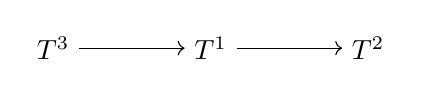
\begin{tikzpicture}[node distance=2cm]
	\node (t3) {$T^3$};
	\node[right of=t3] (t1) {$T^1$};
	\node[right of=t1] (t2) {$T^2$};
	\draw[->] (t3) -- (t1);
	\draw[->] (t1) -- (t2);
\end{tikzpicture}

\begin{enumerate}[i)]
	\item
	Acyclic dependency graph
	$\Rightarrow$ conflict-serializable.

	Equivalent serial schedule:
	$T^3 \rightarrow T^1 \rightarrow T^2$.
\end{enumerate}

\item $S_2$:

Conflicting operations:
\begin{itemize}
	\item $w_3(y)$ before $r_4(y)$ on item $y$
\end{itemize}

Dependency graph $S_2$: \newline
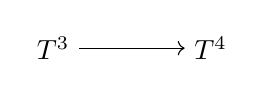
\begin{tikzpicture}[node distance=2cm]
	\node (t3) {$T^3$};
	\node[right of=t3] (t4) {$T^4$};
\draw[->] (t3) -- (t4);
\end{tikzpicture}

\begin{enumerate}[i)]
	\item
	Acyclic dependency graph
	$\Rightarrow$ conflict-serializable.

	Equivalent serial schedule:
	$T^1 \rightarrow T^2 \rightarrow T^3 \rightarrow T^4$.
\end{enumerate}

\item $S_3$:

Conflicting operations:
\begin{itemize}
	\item $r_2(w)$ before $w_1(w)$ on item $w$
	\item $w_3(x)$ before $w_2(x)$ on item $x$
	\item $w_2(x)$ before $w_4(x)$ on item $x$
	\item $w_2(y)$ before $w_5(y)$ on item $y$
	\item $r_1(v)$ before $w_5(v)$ on item $v$
	\item $w_5(v)$ before $w_4(v)$ on item $v$
\end{itemize}

Dependency graph $S_3$: \newline
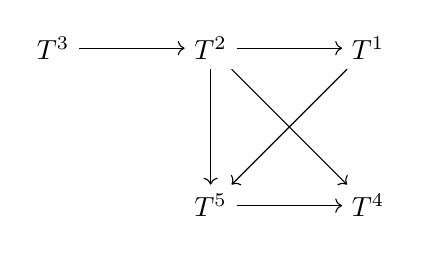
\begin{tikzpicture}[node distance=2cm]
	\node (t3) {$T^3$};
	\node[right of=t3] (t2) {$T^2$};
	\node[right of=t2] (t1) {$T^1$};
	\node[below of=t2] (t5) {$T^5$};
	\node[right of=t5] (t4) {$T^4$};

	\draw[->] (t3) -- (t2);
	\draw[->] (t2) -- (t1);
	\draw[->] (t2) -- (t5);
	\draw[->] (t1) -- (t5);
	\draw[->] (t2) -- (t4);
	\draw[->] (t5) -- (t4);
\end{tikzpicture}

\begin{enumerate}[i)]
	\item
	Acyclic dependency graph
	$\Rightarrow$ conflict-serializable.

	Equivalent serial schedule:
	$T^3 \rightarrow T^2 \rightarrow T^1 \rightarrow T^5 \rightarrow T^4$.
\end{enumerate}

\end{enumerate}


\task{}
\begin{enumerate}[i]
  \item Parameters given in the sheet:\\
    \begin{tabular}{|c|c|c|} \hline \textbf{Parameter} & \textbf{Symbol} & \textbf{Value} \\ \hline 
      Attribute size & $s_{\text{a}}$ & 6 B \\ 
      Tuple size & $s_{\text{t}}$ & 12 B \\
      Cardinality of R & Card(R) & 50\,000 \\ 
      Page size & page & 8192 B \\ 
      Fill degree (data pages) & $f_{\text{data}}$ & 0.9 \\ 
      Fill degree (index pages) & $f_{\text{index}}$ & 0.7 \\ 
      Page header & head & 48 B \\  
      Pointer size & $s_{\text{p}}$ & 6 B \\
      \hline \end{tabular}
  \item \textbf{FF(A)}\\
    Attribute A is uniformly distributed in [0..999], therefore $\mathbf{FF(A=a)=1/1000}$.

  \item \textbf{FF(B)}\\
    Attribute $B$ is not uniformly distributed:\\
    - $40\,000$ tuples are uniformly distributed over the values $[0..99]$ (100 values)\\
    The tuples are spread uniformly across $100$ values so each value occurs $\frac{40\,000}{100} = 400$ times.\\
    Therefore $\mathbf{FF(B = 10) = \frac{400}{50\,000}}$.\\
    - $10\,000$ tuples are uniformly distributed over the values $[100..999]$ (900 values)\\
    Here the tuples are spread uniformly across $900$ different values so each value occurs $\frac{10\,000}{900} \approx 11.11$ times.\\
    Therefore $\mathbf{FF(B = 500) = \frac{10\,000/900}{50\,000}}$.
\end{enumerate}

\begin{enumerate}

\item \textbf{No index (Layout R)}

Page-layout:
$\frac{(\text{page} - \text{head}) \cdot f_{\text{data}}}{r_{\text{avg}} + p_{\text{slot}}} \Longrightarrow \underline{x = 407} $ \\ 
(with $r_{\text{avg}} = s_t$ and $p_{\text{slot}} = s_p$)

Number of data pages: 
$\lceil Card(R) / x \rceil \Longrightarrow \underline{NPages(R) = 123} $

Since there is no index:
$\mathbf{\Longrightarrow C(A=10) = C(A=500) = C(B=10) = C(B=500) = 123}$

\item \textbf{Indirect B+ tree on A (Layout RA)}

Leaf capacity:
$ \left\lceil \frac{(page - head - 2 \cdot p_{leaf})\cdot f_{\text{index}}}{k + r_k \cdot p_{rec}} \right\rceil \Longrightarrow \underline{t_{\text{leaf}} = 18} $\\
(with $k = s_a$, $r_k = 50, p_{leaf} = p_{rec} = s_p $ )

Number of leaf pages: 
$\lceil \frac{n_k}{t_{\text{leaf}}} \rceil \Longrightarrow \underline{n_{\text{leaf}} = 56}$\\
(with $n_k = 1000$)

Inner node capacity: 
$\left\lceil \frac{((page - head)\cdot f_{\text{index}}) - p}{k + p} \right\rceil \Longrightarrow \underline{e_i = 474}$\\
(with $p = s_p$)

Height:
$\lceil \log_{e_i + 1}(n_{\text{leaf}})\rceil + 1  \Longrightarrow \mathbf{h = 2}$

Index-only selection cost: 
$ (h - 1) + \lceil FF(A=a)\cdot n_{\text{leaf}} \rceil \Longrightarrow \mathbf{C(A=10)=C(A=500)=2 }$

Queries on B require table scan:
$ \Longrightarrow \mathbf{C(B=10)=C(B=500)=123} $

\newpage

\item \textbf{Indirect B+ tree on B (Layout RB)}

The index structure parameters are the same as RA:\\
$\Longrightarrow \underline{t_{\text{leaf}} = 18,\ n_{\text{leaf}} = 56,\ e_i = 474,\ }$

Height:
$\lceil \log_{e_i + 1}(n_{\text{leaf}})\rceil + 1  \Longrightarrow \mathbf{h = 2}$

Queries on A require table scan:
$ \Longrightarrow \mathbf{C(A=10)=C(A=500)=123 }$

Index-only selection cost: 
$ (h - 1) + \lceil FF(B=b)\cdot n_{\text{leaf}} \rceil \Longrightarrow \mathbf{C(B=10)=C(B=500)=2 }$

\item \textbf{Two indirect indexes on A and B (Layout RAB)}

Both RA and RB exist.

Heights and Cost identical (to calculation of indexes):\\
$\Longrightarrow \mathbf{h=2}$\\ 
$\Longrightarrow \mathbf{C(A=10)=C(A=500)=2}$ \\
$\Longrightarrow \mathbf{C(B=10)=C(B=500)=2}$

\item \textbf{Clustered, direct index on A (Layout RA\$)}

Means physically sorted by A $\rightarrow$ Leaf pages = table pages.

The parameters are the same as before:\\
$\Longrightarrow \underline{x = 407,\ n_{\text{leaf}} \rightarrow NPages(R) = 123,\ e_i = 474,\ }$

Height:
$\lceil \log_{e_i+1}(n_{\text{leaf}}) \rceil + 1 \Longrightarrow \mathbf{h = 2}$

Cost for A:
$ (h - 1) + \lceil FF(A=a)\cdot n_{\text{leaf}} \rceil \Longrightarrow \mathbf{C(A=10)=C(A=500)=2 }$\\
B has no usable index:
$\Longrightarrow \mathbf{ C(B=10)=C(B=500)=123 }$

\item \textbf{Combined B+ tree on (A,B) (Layout RC)}

Combined search key: 
$ s_A + s_B \Longrightarrow \underline{k = 12}$.

Number of distinct key pairs:
$ 1000 \cdot 1000 \Longrightarrow \underline{n_k = 1\,000\,000}$.

Average number of tuples per key pair:
$ \frac{Card(R)}{n_k} \Longrightarrow \underline{r_k = 0.05}$.

Leaf capacity (page-layout indirect index):
$\left\lceil \frac{(\text{page} - \text{head} - 2 \cdot p_{\text{leaf}})\cdot f_{\text{index}}}{k + r_k \cdot p_{\text{rec}}} \right\rceil
\Longrightarrow \underline{t_{\text{leaf}} = 462}. $

Number of leaf pages:
$
= \left\lceil \frac{n_k}{t_{\text{leaf}}} \right\rceil
 \Longrightarrow \underline{n_{\text{leaf}} = 2165} $

Inner node capacity:
$ \left\lceil \frac{((\text{page} - \text{head})\cdot f_{\text{index}}) - p}{k + p} \right\rceil
\Longrightarrow \underline{e_i = 316}. $

Height of the index:
$ \left\lceil \log_{e_i + 1}(n_{\text{leaf}}) \right\rceil + 1
\mathbf{\Longrightarrow h = 3}$

Cost for queries on $A$:
$ (h - 1) + \left\lceil FF(A = a) \cdot n_{\text{leaf}} \right\rceil
= \mathbf{\Longrightarrow C(A = 10) = C(A = 500) = 5}. $

$B$ alone cannot use the combined index (no leading $A$):
$\mathbf{\Longrightarrow C(B = 10) = C(B = 500) = 123}. $

\end{enumerate}

Summary:\\     
\begin{tabular}{|l||c|c|c|c||c|}
\hline
Layout & A=10 & B=10 & A=500 & B=500 & Height \\ \hline\hline
\texttt{R}   & 123 & 123 & 123 & 123 & no index \\ \hline
\texttt{RA}  & 2   & 123 & 2   & 123 & 2 \\ \hline
\texttt{RB}  & 123 & 2   & 123 & 2   & 2 \\ \hline
\texttt{RAB} & 2   & 2   & 2   & 2   & 2 \\ \hline
\texttt{RA\$}& 2   & 123 & 2   & 123 & 2 \\ \hline
\texttt{RC}  & 5   & 123 & 5   & 123 & 3 \\ \hline
\end{tabular}


\task{}
% -------------------- Task 3a: Schedule S7 --------------------
\noindent\textbf{a) Given schedule:}
\[
S_7=\langle
\ri{2}{a}\;
\ri{1}{b}\;
\wi{1}{b}\;
\ri{1}{a}\;
\ri{4}{b}\;
\Ci{1}\;
\ri{3}{c}\;
\ri{3}{b}\;
\wi{2}{a}\;
\wi{2}{b}\;
\Ci{2}\;
\ri{3}{a}\;
\Ci{3}
\rangle
\]
Committed transactions: $\T{1},\T{2},\T{3}$ (via $\Ci{1},\Ci{2},\Ci{3}$). Transaction $\T{4}$ is \emph{active} (no $C_4/A_4$).

\vspace{0.6em}

\begingroup
\renewcommand{\labelenumi}{(\arabic{enumi})}
\setlength{\leftmargini}{1.8em}

\begin{enumerate}
\item \textbf{CPSR: No.}\\
For conflict-serializability we consider the \emph{committed projection} $C(S_7)$, i.e., remove all actions of non-committed transactions (here: remove $\T{4}$):
\[
C(S_7)=\langle
\ri{2}{a}\;
\ri{1}{b}\;
\wi{1}{b}\;
\ri{1}{a}\;
\Ci{1}\;
\ri{3}{c}\;
\ri{3}{b}\;
\wi{2}{a}\;
\wi{2}{b}\;
\Ci{2}\;
\ri{3}{a}\;
\Ci{3}
\rangle
\]
Serialization graph on committed transactions $\{\T{1},\T{2},\T{3}\}$ has conflict edges:
\begin{itemize}
  \setlength{\itemsep}{0.2em}
  \setlength{\parskip}{0pt}
  \setlength{\parsep}{0pt}
  \item On $b$: $\wi{1}{b}$ before $\ri{3}{b}$ \;$\Rightarrow$ $\T{1}\rightarrow \T{3}$.
  \item On $b$: $\ri{3}{b}$ before $\wi{2}{b}$ \;$\Rightarrow$ $\T{3}\rightarrow \T{2}$.
  \item On $a$: $\wi{2}{a}$ before $\ri{3}{a}$ \;$\Rightarrow$ $\T{2}\rightarrow \T{3}$.
\end{itemize}
Thus there is a cycle $\T{2}\leftrightarrow \T{3}$, hence $S_7\notin\mathrm{CPSR}$.

\item \textbf{RC: Yes.}\\
Reads-from relation:
\begin{itemize}
  \setlength{\itemsep}{0.2em}
  \setlength{\parskip}{0pt}
  \setlength{\parsep}{0pt}
  \item $\ri{3}{b}$ reads from $\wi{1}{b}$ \;$\Rightarrow$ $(\T{1},b,\T{3})\in RF(S_7)$.
  \item $\ri{3}{a}$ reads from $\wi{2}{a}$ \;$\Rightarrow$ $(\T{2},a,\T{3})\in RF(S_7)$.
\end{itemize}
Since $\Ci{1}<\Ci{3}$ and $\Ci{2}<\Ci{3}$, the schedule is recoverable: $S_7\in\mathrm{RC}$.

\item \textbf{ACA: No.}\\
$\ri{4}{b}$ reads the value written by $\wi{1}{b}$ before $\T{1}$ commits:
\[
\wi{1}{b}\;<\;\ri{4}{b}\;<\;\Ci{1},
\]
so a dirty read occurs and $S_7\notin\mathrm{ACA}$.

\item \textbf{ST: No.}\\
Strictness is violated because $\T{4}$ reads $b$ after $\T{1}$ wrote $b$ but before $\T{1}$ commits:
\[
\wi{1}{b}\;<\;\ri{4}{b}\;<\;\Ci{1}.
\]
Hence $S_7\notin\mathrm{ST}$.

\item \textbf{RG: No.}\\
Rigorous requires that between any two conflicting actions the earlier transaction has already terminated.
The conflict $\wi{1}{b} < \ri{4}{b}$ has no $C_1/A_1$ in between, thus $S_7\notin\mathrm{RG}$.
\end{enumerate}

\endgroup

\vspace{0.4em}
\noindent\textbf{Final classification:}
\[
S_7 \notin \mathrm{CPSR},\qquad
S_7 \in \mathrm{RC},\qquad
S_7 \notin \mathrm{ACA},\qquad
S_7 \notin \mathrm{ST},\qquad
S_7 \notin \mathrm{RG}.
\]



\noindent\textbf{b) Given schedule:}
\[
S_8=\langle
\ri{3}{b}\;
\ri{1}{a}\;
\ri{4}{a}\;
\wi{4}{a}\;
\Ci{4}\;
\ri{3}{a}\;
\wi{3}{b}\;
\ri{2}{b}\;
\wi{1}{c}\;
\Ci{1}\;
\ri{2}{c}\;
\wi{2}{b}\;
\ri{3}{b}\;
\Ci{3}\;
\Ai{2}
\rangle
\]
Committed transactions: $\T{1},\T{3},\T{4}$ (via $\Ci{1},\Ci{3},\Ci{4}$). Transaction $\T{2}$ \emph{aborts}.

\vspace{0.6em}

\begingroup
\renewcommand{\labelenumi}{(\arabic{enumi})}
\setlength{\leftmargini}{1.8em}

\begin{enumerate}
\item \textbf{CPSR: Yes.}\\
For conflict-serializability we consider the committed projection $C(S_8)$, i.e., remove all actions of non-committed transactions (here: remove $\T{2}$):
\[
C(S_8)=\langle
\ri{3}{b}\;
\ri{1}{a}\;
\ri{4}{a}\;
\wi{4}{a}\;
\Ci{4}\;
\ri{3}{a}\;
\wi{3}{b}\;
\wi{1}{c}\;
\Ci{1}\;
\ri{3}{b}\;
\Ci{3}
\rangle
\]
Serialization graph on committed transactions $\{\T{1},\T{3},\T{4}\}$ has conflict edges:
\begin{itemize}
  \setlength{\itemsep}{0.2em}
  \setlength{\parskip}{0pt}
  \setlength{\parsep}{0pt}
  \item On $a$: $\ri{1}{a}$ before $\wi{4}{a}$ \;$\Rightarrow$ $\T{1}\rightarrow \T{4}$.
  \item On $a$: $\wi{4}{a}$ before $\ri{3}{a}$ \;$\Rightarrow$ $\T{4}\rightarrow \T{3}$.
\end{itemize}
There are no other conflicts among $\T{1},\T{3},\T{4}$, and the graph is acyclic (order $\T{1}\rightarrow\T{4}\rightarrow\T{3}$).
Hence $S_8\in\mathrm{CPSR}$.

\item \textbf{RC: No.}\\
Reads-from relation (relevant reads):
\begin{itemize}
  \setlength{\itemsep}{0.2em}
  \setlength{\parskip}{0pt}
  \setlength{\parsep}{0pt}
  \item $\ri{3}{a}$ reads from $\wi{4}{a}$ \;$\Rightarrow$ $(\T{4},a,\T{3})\in RF(S_8)$.
  \item $\ri{2}{c}$ reads from $\wi{1}{c}$ \;$\Rightarrow$ $(\T{1},c,\T{2})\in RF(S_8)$.
  \item $\ri{2}{b}$ reads from $\wi{3}{b}$ \;$\Rightarrow$ $(\T{3},b,\T{2})\in RF(S_8)$.
  \item The later $\ri{3}{b}$ reads from $\wi{2}{b}$ \;$\Rightarrow$ $(\T{2},b,\T{3})\in RF(S_8)$.
\end{itemize}
Transaction $\T{3}$ commits ($\Ci{3}$) but reads $b$ from $\T{2}$, and $\T{2}$ does \emph{not} commit (it aborts: $\Ai{2}$).
Therefore the schedule is not recoverable: $S_8\notin\mathrm{RC}$.

\item \textbf{ACA: No.}\\
A dirty read occurs: $\ri{2}{b}$ reads the value written by $\wi{3}{b}$ before $\T{3}$ commits:
\[
\wi{3}{b}\;<\;\ri{2}{b}\;<\;\Ci{3}.
\]
Hence $S_8\notin\mathrm{ACA}$.

\item \textbf{ST: No.}\\
Strictness is violated because after $\T{3}$ writes $b$, another transaction reads $b$ before $\T{3}$ commits:
\[
\wi{3}{b}\;<\;\ri{2}{b}\;<\;\Ci{3}.
\]
(Also, $\wi{2}{b}<\ri{3}{b}<\Ai{2}$ violates strictness as well.)
Thus $S_8\notin\mathrm{ST}$.

\item \textbf{RG: No.}\\
Rigorous requires that between any two conflicting actions the earlier transaction has already terminated.
The conflict $\wi{3}{b}<\ri{2}{b}$ has no $C_3/A_3$ in between, hence $S_8\notin\mathrm{RG}$.
\end{enumerate}

\endgroup

\vspace{0.4em}
\noindent\textbf{Final classification (S8):}
\[
S_8 \in \mathrm{CPSR},\qquad
S_8 \notin \mathrm{RC},\qquad
S_8 \notin \mathrm{ACA},\qquad
S_8 \notin \mathrm{ST},\qquad
S_8 \notin \mathrm{RG}.
\]


\end{document}
